\documentclass{beamer}
% \usepackage{animate}
\usepackage{multimedia}
\usepackage[english,russian]{babel}

\usepackage{pgfpages}
\setbeameroption{show notes on second screen}
%https://tug.ctan.org/macros/latex/contrib/beamer/doc/beameruserguide.pdf

\usepackage[T2A]{fontenc}
\usepackage[utf8]{inputenc}

\setbeamertemplate{caption}[numbered]

\usetheme{CambridgeUS}
\usecolortheme{dolphin}


\title[Image Rendering Technologies]{Технологии рендеринга изображений}
\author[Быковских Д.А.]{Быковских Дмитрий Александрович}
\date{14.12.2024}


\begin{document}

	\begin{frame}
		\titlepage
	\end{frame}

	\begin{frame}{Введение}

		Технологии рендеринга изображений представляют собой разнообразные модели, методы, алгоритмы, подходы и инструменты для построения (или создания) изображений из трёхмерных (или двумерных) сцен.

		Технологии построения изображений включают:
		\begin{itemize}
			\item модели освещения;
			\item методы визуализации;
			\item техники освещения и алгоритмы;
			\item аппаратно-программные средства.
		\end{itemize}

		\note{
		
		}

	\end{frame}

	\begin{frame}{Модели освещения}

		Модель освещения --- математическое представление процесса взаимодействия света с поверхностями объектов в сцене.
		
		\begin{figure}
			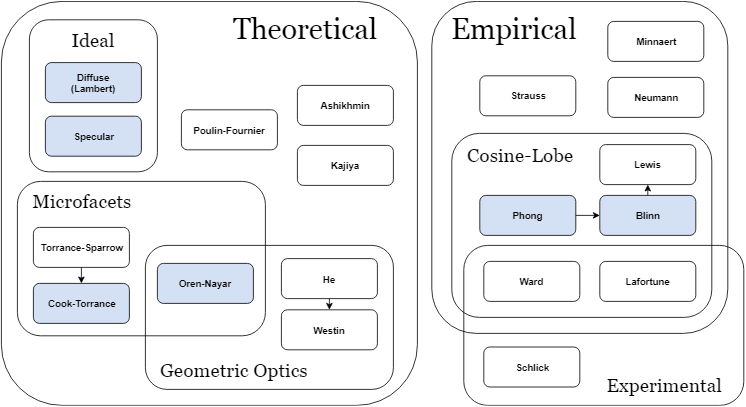
\includegraphics[width=0.8\textwidth]{images/lightning-model-scheme.png}
			\caption{
				\href{https://cglearn.eu/pub/advanced-computer-graphics/physically-based-shading}{Классификация моделей освещения}
				% \href{https://digibug.ugr.es/bitstream/handle/10481/19751/rmontes_LSI-2012-001TR.pdf}{Классификация моделей освещения}
			}
		\end{figure}

		
		\note{
			Модели освещения описывают физические процессы излучения, отражения (рассеяния), преломления и поглощения света.

			Фактически модели освещения определяют, как свет влияет на внешний (визуальный) вид объектов.

			Модели освещения можно разделить на:
			\begin{itemize}
				\item эмпирические;
				\item физически обоснованные (Physically-Based Rendering или PBR);
				\item специализированные.
			\end{itemize}
		
		}
	
	\end{frame}

	
	\begin{frame}{Эмпирические модели освещения}

		\footnotesize

		\begin{itemize}
			\item 
			Ламбертово освещение (Lambertian Reflectance, 1760-е, И.~Г.~Ламберт)\\
			Модель для диффузного отражения, где интенсивность света зависит от угла между нормалью поверхности и направлением света.\\
			{Источник:} «Photometria», J.~H.~Lambert, 1760.

			\item 
			Фонг (Phong Shading, 1975 г., Б.~Т.~Фонг)\\
			Диффузное и спекулярное освещение.\\
			Использует эмпирическую формулу для блеска.\\
			\href{https://users.cs.northwestern.edu/~ago820/cs395/Papers/Phong_1975.pdf}{Illumination for computer-generated pictures, B.~T.~Phong, 1975.}

			\item 
			Блинн-Фонг (Blinn-Phong, 1977 г., Д.~Ф.~Блинн)\\
			Упрощение модели Фонга с использованием полувектора для расчёта бликов.\\
			{Источник:} «Models of Light Reflection for Computer Synthesized Pictures», J.~F.~Blinn, 1977.

			\item 
			Льюис (Lewis Model, 1983 г., Д.~Льюис)\\
			Упрощённая модель освещения для интерактивных приложений. Стала популярна благодаря производительности и гибкости.\\
			{Источник:} Распространена в материалах индустрии компьютерной графики.

		\end{itemize}

		\note{

			% Эмпирический --- термин, означающий основанный на опыте, наблюдении или экспериментах, но не на строгих теоретических или физических законах. 

			% \vspace{0.15cm}

			Модель освещения Блинна-Фонга
			\[
				I = k_e + I_a k_a + \sum_{j=1}^{m} \frac{I_{j}}{d+k} \bigg[ k_d (N_j \cdot L_j) + k_s (N_j \cdot H)^{\alpha_j} \bigg]
			\]

			\begin{figure}
				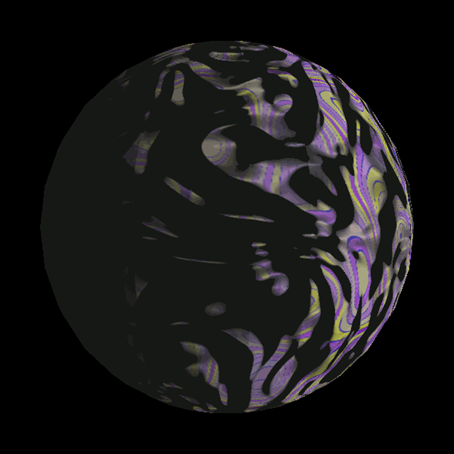
\includegraphics[width=0.35\textwidth]{images/rasterization-example.png}
				\caption{
					 Модель освещения Блинна-Фонга и растеризатор
					}
			\end{figure}

		}
	\end{frame}
	
	
	\begin{frame}{Физически обоснованные модели освещения (Physically-Based Rendering Technique или PBRT)}

		% \footnotesize

		\begin{itemize}
			\item 
			Кук-Торранс (Cook-Torrance, 1982 г., Р. Кук и К. Торранс)\\
			Учитывает микрофасетки поверхности, описывая отражение с помощью BRDF.\\
			Включает микрофацетную нормаль (модель GGX или Бекмана).\\
			Источник: «A Reflectance Model for Computer Graphics», Cook~Torrance, 1982
	
			\item
			Орен-Наяр (Oren-Nayar, 1994 г., М. Орен и Ш. Наяр)\\
			Расширение ламбертовой модели для шероховатых поверхностей.\\
			Источник: «Generalization of Lambert's Reflectance Model», Oren~and~Nayar, 1994
	
			\item 
			Шлик (Schlick Approximation, 1994 г., К. Шлик)\\
			Апроксимация уравнения Френеля для отражения света.\\
			Источник: «An Inexpensive BRDF Model for Physically-based Rendering», Christophe Schlick, 1994
		
		\end{itemize}

		\note{

			Пример модели освещения, использующей PBRT
			\[
				L_o(x, \omega_o) = 
				L_e(x, \omega_o) + 
				\int_{\Omega} 
				\frac{D(h) F(h, \omega_o) G(x, \omega_o, \omega_i)}{4 (\omega_o \cdot n) (\omega_i \cdot n)} 
				L_i(x, \omega_i) \max(0, n \cdot \omega_i) \, d\omega_i
			\]

			\begin{figure}
				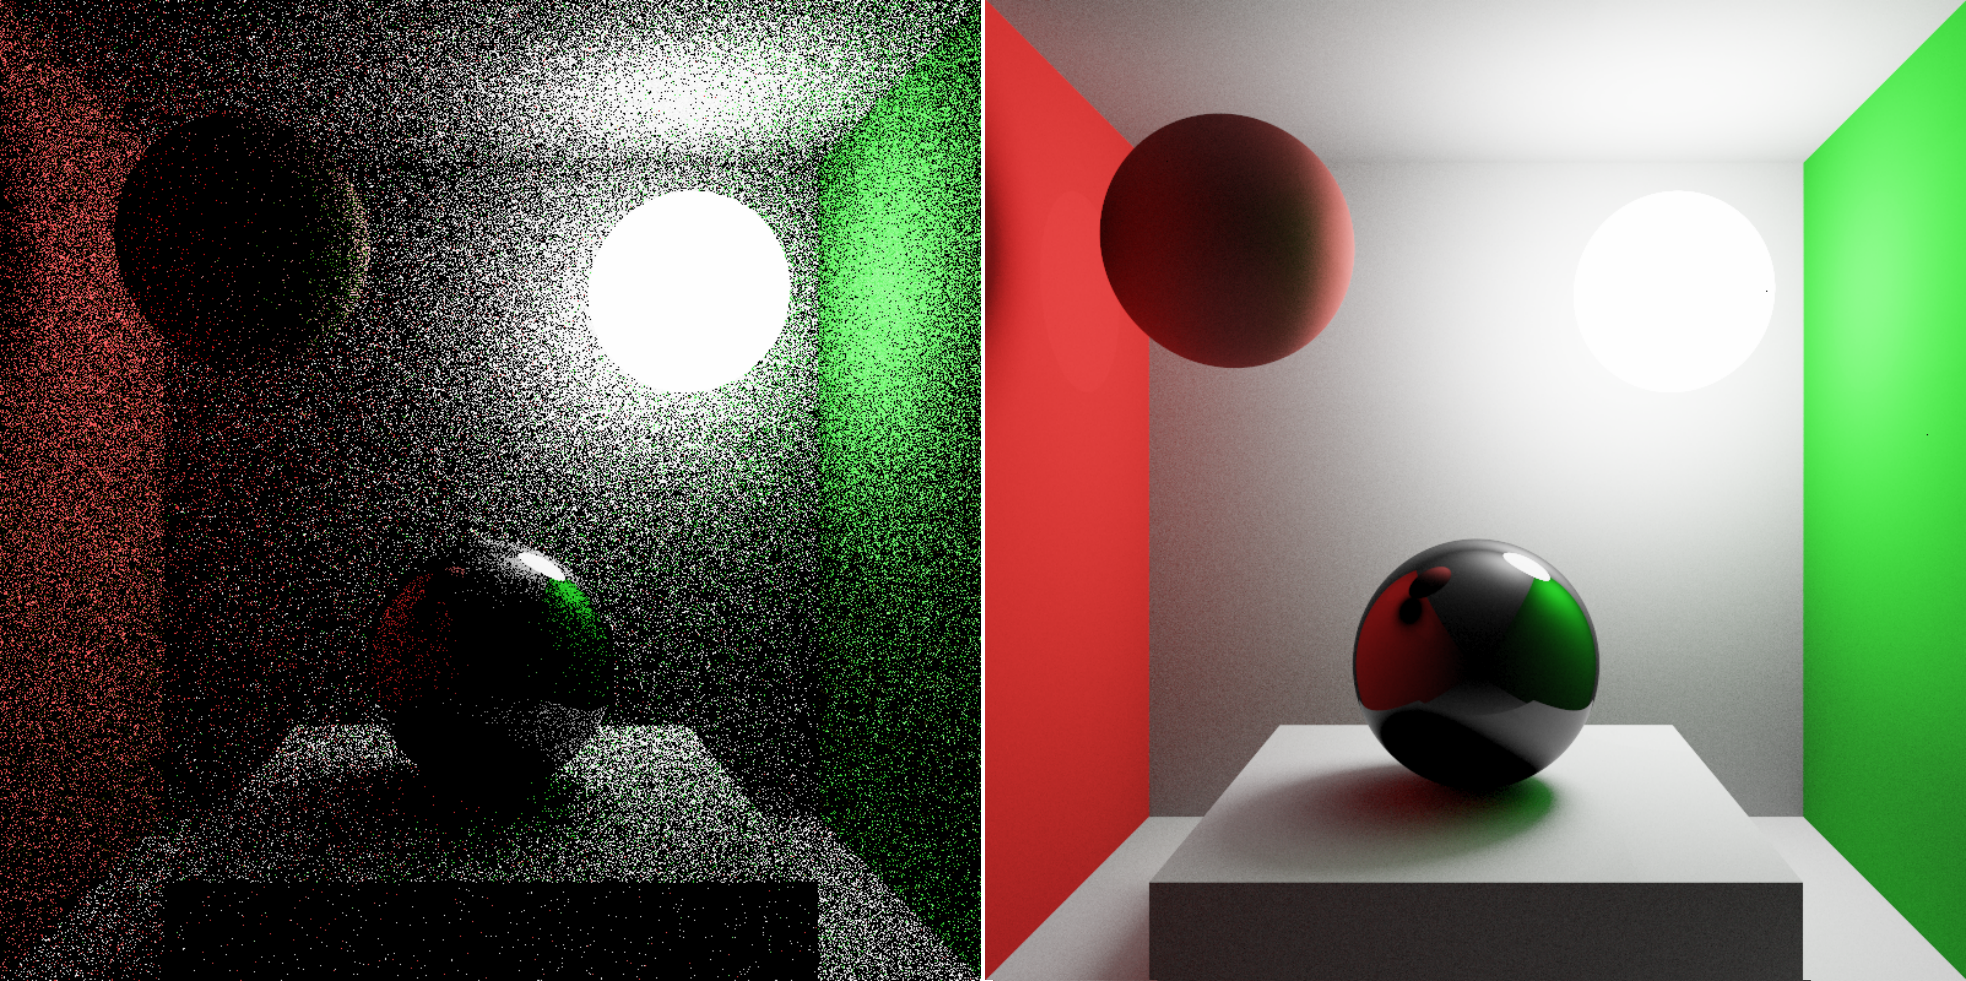
\includegraphics[width=0.7\textwidth]{images/path-tracing-example.png}
				\caption{
					Модель освещения, использующая PBRT, и метод трассировки пути
					}
			\end{figure}

			% \scriptsize
			% Примечание.

			% Физически-корректные или
			% Физически-обоснованные

		}

	\end{frame}


	\begin{frame}{
		Современные модели освещения, основанные на PBRT
		}

		\begin{itemize}
			\item 
			Дисней (Disney BRDF, 2012 г., Walt Disney Animation Studios)\\
			Обобщённая модель PBR, разработанная в Walt Disney Animation Studios.\\
			{Источник:} \href{https://media.disneyanimation.com/uploads/production/publication_asset/48/asset/s2012_pbs_disney_brdf_notes_v3.pdf}{Physically Based Shading at Disney, Brent Burley, 2012.}
	
			\item 
			Autodesk Standard Surface\\
			Универсальная модель поверхностей, используемая в индустрии для физически корректного рендеринга.\\
			{Источник:} \href{https://autodesk.github.io/standard-surface/}{Документация Autodesk Standard Surface, I.~Georgiev et al., 2019~г.}
	
			\item 
			Принципиальный BSDF (Principled BSDF) в Blender\\
			Шейдер для удобного использования PBR-материалов в Blender, основанный на Disney BRDF.\\
			{Источник:} \href{https://docs.blender.org/manual/ru/4.3/render/shader_nodes/shader/principled.html}{Документация Blender, Principled BSDF.}
	\end{itemize}

	\note{
		\begin{figure}
			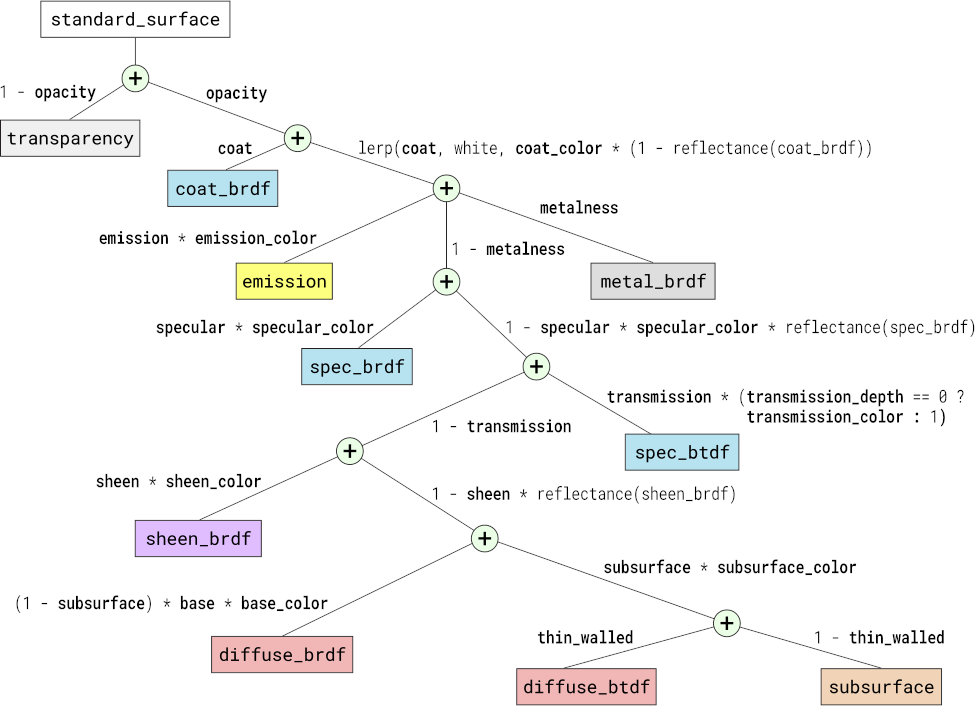
\includegraphics[width=0.7\textwidth]{images/autodesk-standard-surface.png}
			\caption{
				\href{https://autodesk.github.io/standard-surface/}{Иерархическое дерево коэффициентов универсальной модели освещения (Autodesk Standard Surface)}
			}
		\end{figure}
	}

	\end{frame}


	\begin{frame}{Специализированные модели}
		\footnotesize

		\begin{itemize}
			\item 
			Шейдеры NPR (Non-Photorealistic Rendering, 1990-е)\\
			Для стилизованных эффектов, таких как Toon Shading.\\
			{Источник:} Основы заложены в 1990-х для мультфильмов и графики.
	
			\item 
			SSS (Subsurface Scattering, 2001 г., Хенрик Ванке)\\
			Освещение полупрозрачных материалов.\\
			{Источник:} \href{https://graphics.stanford.edu/papers/bssrdf/bssrdf.pdf}{«A Practical Model for Subsurface Light Transport», Jensen, 2001}.
	
			\item 
			Объёмное освещение (Volumetric Lighting, 1990-е)\\
			Имитация взаимодействия света с объёмными средами.\\
			{Источник:} Применение в движках RenderMan.
	
			\item 
			Рендеринг волос (Hair Rendering, 2003 г., Маркос Фажардо)\\
			Специфические модели освещения и самозатенения для реалистичной симуляции волос.\\
			{Источник:} \href{https://www.cs.cornell.edu/~srm/publications/SG06-hair.pdf}{«Rendering Hair Using a Photon Mapping Approach», Marschner et~al., 2003.}
	
			% \item 
			% Теневые карты (Shadow Mapping, 1978 г., Ланс Уильямс)\\
			% Расчёт теней с помощью глубинного буфера.\\
			% [Источник: «Casting Curved Shadows on Curved Surfaces», Lance Williams, 1978]
	
			% \item 
			% AO (Ambient Occlusion, 1998 г.)\\
			% Подсветка скрытых областей для усиления реализма.\\
			% [Источник: «Introduction to Ambient Occlusion», Simon Green, 2002]
		\end{itemize}

		\note{
			\begin{figure}
				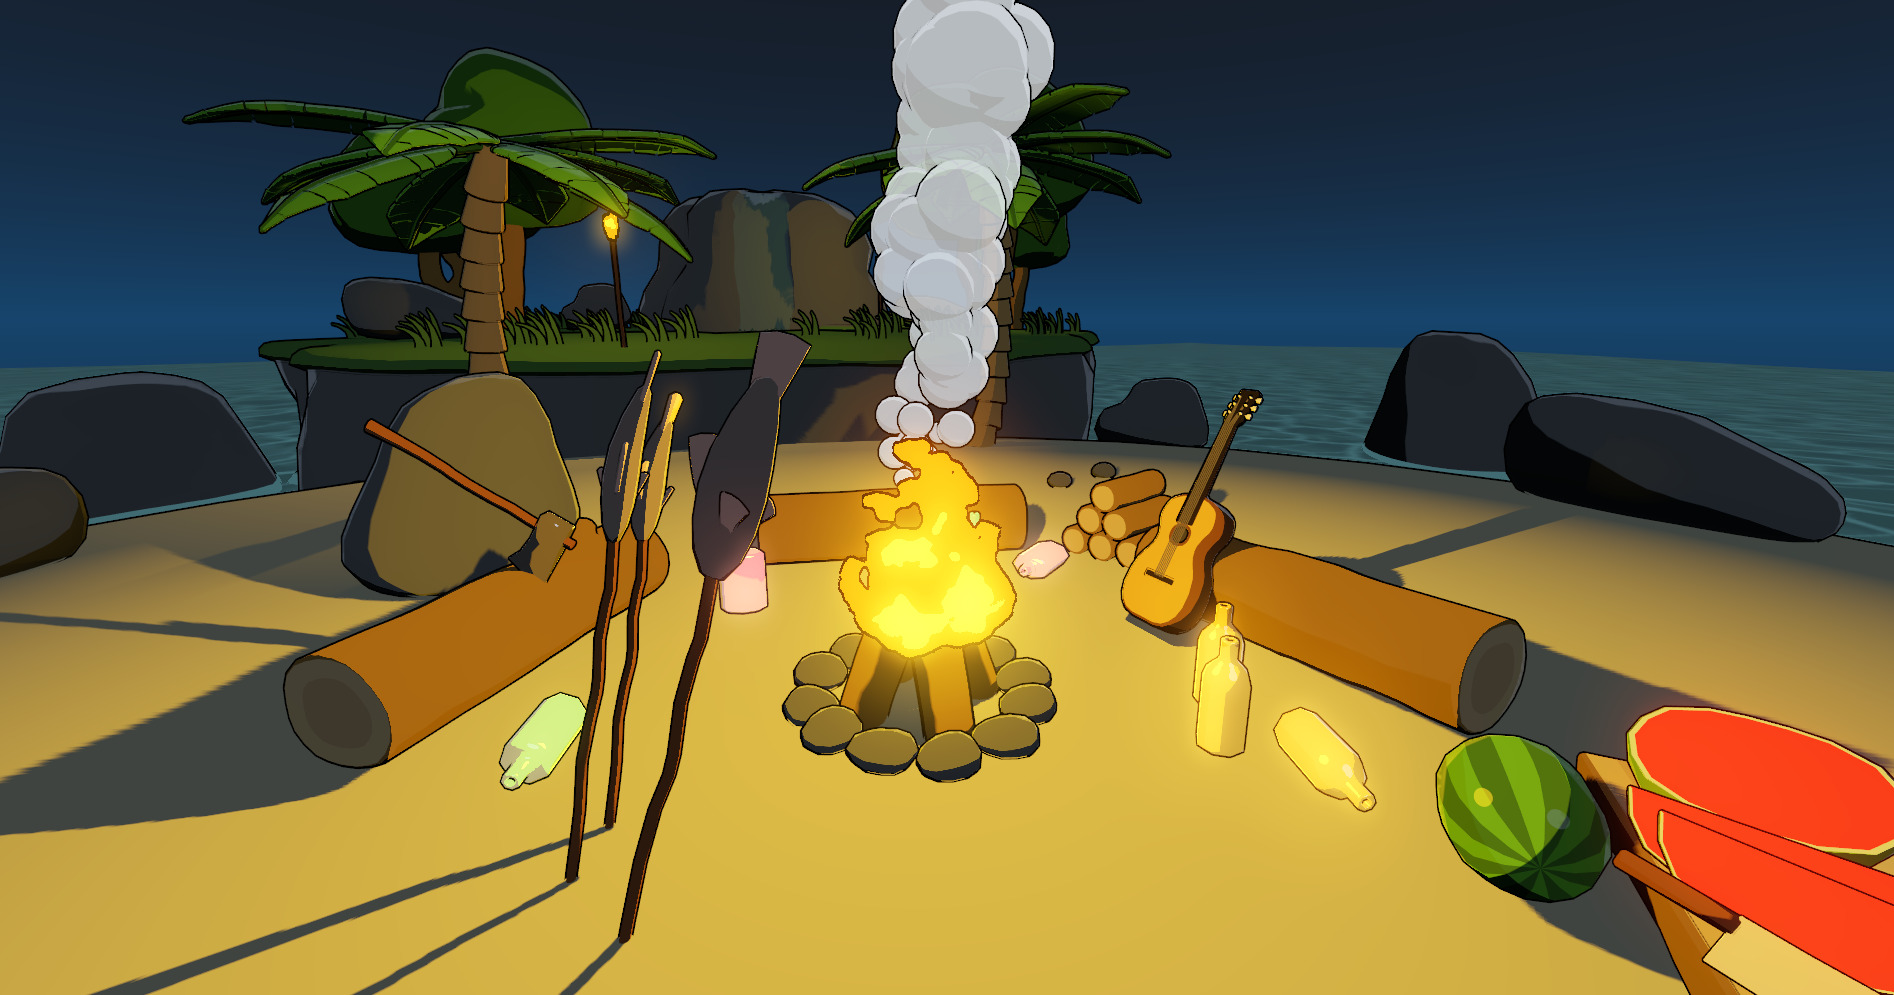
\includegraphics[width=0.75\textwidth]{images/toon-shader.jpg}
				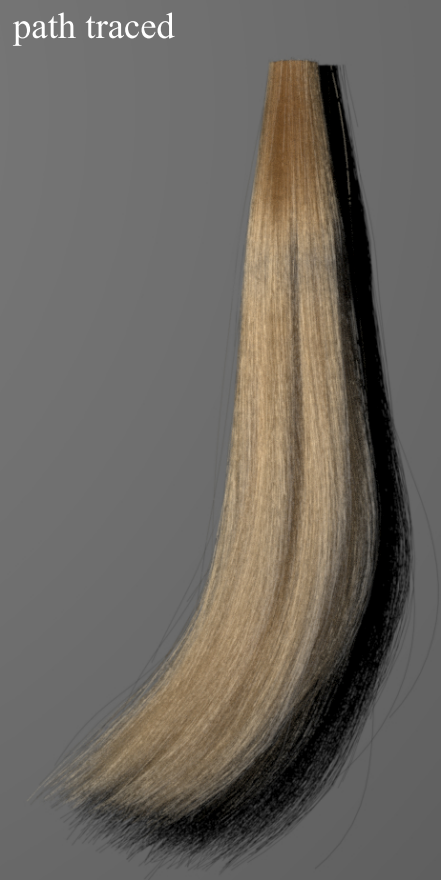
\includegraphics[width=0.22\textwidth]{images/hair-rendering.png}
				\caption{
					\href{https://godotshaders.com/shader/complete-toon-shader/}{Изображения, полученные с помощью Toon Shading (слева) и Hair Rendering (справа)}
				}
			\end{figure}
		}
	\end{frame}

	\if 0
	\begin{frame}{Введение}
	
		Модель освещения --- математическое представление процесса взаимодействия света с поверхностями и объектами в сцене.\\
		{\footnotesize
		Модели освещения описывают физические процессы отражения, преломления, рассеяния и поглощения света.\\
		Модели освещения определяют, как свет влияет на визуальный внешний вид объектов. (сравнить)
		}

		\vspace{0.15cm}

		Метод (Method в контексте компьютерной графики) --- способ вычисления или приближенного вычисления освещения, используя различные математические подходы.\\
		{\footnotesize
		С одной стороны, методы часто используют те или иные модели освещения для получения итогового результата. 
		С другой стороны, метод может включать несколько техник и алгоритмов для вычисления освещения на сцене.
		}
		
		\vspace{0.15cm}
		Техника освещения --- конкретный способ применения модели или метода освещения в практике. \\
		{\footnotesize
		Техники освещения могут включать дополнительные механизмы, которые ускоряют процесс рендеринга или помогают достичь определенных визуальных эффектов. 
		Техники обычно привязаны к специфическим алгоритмам и инструментам.
		}
		
		\vspace{0.15cm}

		Алгоритм --- последовательность шагов, предназначенная для решения определенной задачи.
		\\
		{\footnotesize
		В графике алгоритм описывает процесс, с помощью которого методы или техники реализуются на практике, в виде математические формул и операций, используя вычислительные системы.
		}

		\note{
		}
		
	\end{frame}
	\fi


	\begin{frame}{Методы визуализации}
		
			
		Метод (в контексте компьютерной графики) --- способ вычисления или приближенного вычисления освещения, используя различные математические подходы.\\

		Виды
		\begin{itemize}
			\item Ray Casting (Метод «бросания лучей»)
			\item Rasterization (Растеризация)
			\item Ray Tracing (Трассировка лучей)
			\item Path Tracing (Трассировка путей)
			\item Photon Mapping (Метод фотонных карт)
			\item Radiosity %(Метод радиозности) добавить
		\end{itemize}
		
		\vspace{0.15cm}
		\scriptsize
		Примечание. 

		Растеризация --- лучший выбор для построения изображений в реальном времени, где важна скорость.

		Трассировка лучей --- промежуточный вариант, баланс между реализмом и производительностью.

		Трассировка путей --- идеальный выбор для фотореалистичных визуализаций, но практически непригоден для построения изображений в реальном времени.

		\note{
			\vspace{0.15cm}
		
			С одной стороны, методы часто используют те или иные модели освещения для получения итогового результата. 
			С другой стороны, метод может включать несколько техник и алгоритмов для вычисления освещения на сцене.

			\vspace{0.15cm}

			Техника освещения --- конкретный способ применения модели и/или метода освещения в практике. \\
			
			Техники освещения могут включать дополнительные механизмы, которые ускоряют процесс рендеринга или помогают достичь определенных визуальных эффектов. 
			Техники обычно привязаны к специфическим алгоритмам и инструментам.
			
			
			\vspace{0.1cm}
	
			Алгоритм --- последовательность шагов, предназначенная для решения определенной задачи.
	
			В графике алгоритм описывает процесс, с помощью которого методы или техники реализуются на практике, в виде математических формул и операций, используя вычислительные системы.

		}
		
	
	\end{frame}

	\begin{frame}{Метод «бросания лучей» (Ray Casting)}

		Ray Casting (или метод «бросания лучей») --- технология, которая преобразует ограниченный набор данных (упрощенная двумерная карта) в 3D проекцию путем «бросания лучей» из точки обзора по всей области видимости.

		\begin{figure}
			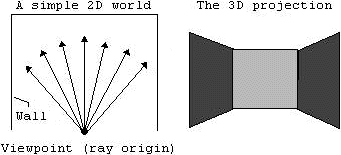
\includegraphics[width=0.55\textwidth]{images/ray-casting.png}
			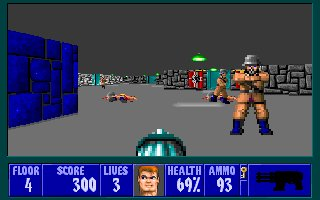
\includegraphics[width=0.4\textwidth]{images/wolf3d.jpg}
			\caption{
				\href{https://habr.com/ru/articles/515256/}{Схема построения изображения с помощью Ray Casting (слева); кадр игры Wolfenstein 3D (1992 г.)(справа)}
			}
		\end{figure}
		
		\note{
			Особенности
			\begin{itemize}
				\item 
				В 1968 г. Артур Аппель (A.~Appel) из IBM описал первую версию Ray~Casting в своей статье о генерации скрытых линий и поверхностей
				(A Technique for Determining Paths and Visibility in Realistic Images).
				\item 
				Высокая скорость построения изображений, поэтому использовался в ранних трехмерных играх.
				\item 
				Отсутствие отражений, теней и глобального освещения.
			\end{itemize}
			
		}

	\end{frame}

	\begin{frame}{Растеризация (Rasterization)}
	
		Растеризация --- метод рендеринга, который преобразует 3D-сцену в 2D-изображение, отображаемое на экране. 
		Этот метод долгое время являлся основным подходом в компьютерной графике для создания изображения в реальном времени 
		и отличается высокой производительностью, так как оптимизирован для работы на GPU.

		\begin{figure}
			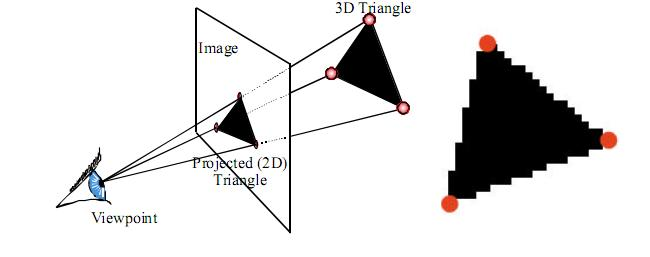
\includegraphics[width=0.75\textwidth]{images/rasterization.jpg}
			\caption{
				\href{https://racketboy.com/retro/about-video-games-rasterization-and-z-buffer}{Схема построения изображения с помощью rasterization}
			}
		\end{figure}

		\note{

			\href{https://www.etymonline.com/word/raster#etymonline_v_36914}{Растер}
			(Raster, 1934) --- сканирующее поле.

			В 1980 году T.~Whitted расширил концепцию Ray Casting, добавив расчет вторичных лучей для отражений и теней.

			\href{https://dl.acm.org/doi/pdf/10.1145/358876.358882}{«An improved illumination model for shaded display», T.~Whitted, 1980.} 

			Недостаток такого метода рендеринга заключается в том, что необходимо использовать дополнительно методы для создания теней и отражений.

		}

	\end{frame}

	\if 0
	\begin{frame}{Тени}

		1. Проецирование теней (Shadow Projection)

		2. Z-буферные тени (Shadow Mapping)

		2.1.	PCF (Percentage-Closer Filtering).% Сглаживание краёв теней.
			
		2.2.	Cascaded Shadow Maps (CSM). % Деление сцены на области с разным разрешением теней.

		3. Объёмные тени (Shadow Volumes)

		4. Screen Space Shadows (SSS)

		5. Тени на основе глобального освещения

		5.1.	Ambient Occlusion (AO)%. Области, куда попадает меньше рассеянного света.

		5.2.	Global Illumination (GI)%. Учёт непрямых источников света.
		
	\end{frame}


	\begin{frame}{Отражения}

		1. Плоские отражения (Planar Reflections)

		2. Кубические карты (Cube Mapping)

		3. Экранные отражения (Screen Space Reflections, SSR)

		4. Ray Traced Reflections

		5. Обратные отражения (Inverse Reflections)

		6. Отражения в глобальном освещении

		7. Light Probes%. Предварительно вычисленные точки с информацией об окружающем освещении.

		8. Photon Mapping%. Просчёт отражённого света через трассировку фотонов.

	\end{frame}

	\fi

	\begin{frame}{Трассировка лучей (Ray Tracing)}
		
		Метод трассировки лучей моделирует распространение света от камеры (наблюдателя) к объектам в сцене и далее к источникам света. 
		Для каждого пикселя изображения отправляется виртуальный «луч» через сцену, чтобы определить, что видит камера в этом направлении.

		\begin{figure}
			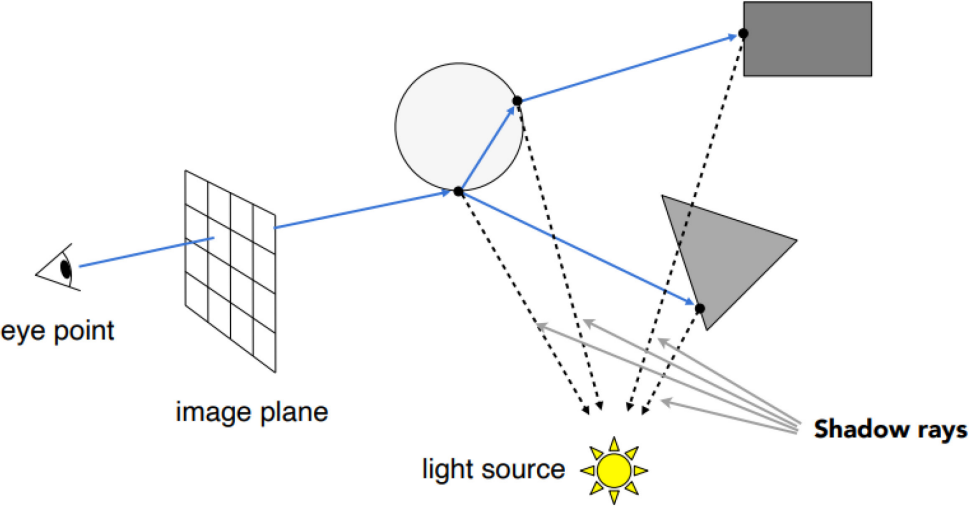
\includegraphics[width=0.65\textwidth]{images/ray-tracing.png}
			\caption{
				\href{https://cglearn.eu/pub/computer-graphics/ray-tracing-space-partitioning-bvh}{Схема траектории движения луча в методе трассировки лучей}
			}
		\end{figure}

		\note{
			\footnotesize

			Шаги процесса

			1. Генерация первичных лучей (primary rays). 
			
			Лучи отправляются из точки зрения камеры через каждый пиксель экрана.

			2. Определение точек пересечения.
			
			Для каждого такого луча проверяется, с какими объектами пересекается его траектория движения, и выбирается ближайшая точка пересечения, которая принадлежит поверхности объекта.

			3. Генерация дополнительных лучей\dots

			3.1. если поверхность отражающая и/или преломляющая (прямое освещение, shadow rays).
			
			3.2. к источникам света для определения степени затенения (косвенное освещение, secondary rays).
			% , при этом, если материал поверхности имеет ненулевую:
			% зеркальную составляющую, то генерируются отражённые лучи
			% прозрачную составляющую --- преломлённые лучи;
			% диффузную составляющую, то --- рассеянные лучи

			% 3. Определение вклада каждого источника света и многократных отражений на основе уравнения рендеринга за счет генерации дополнительных лучей

			Луч перестает отслеживаться, после: его поглощения, выхода за границу сцены или при достижении заданного числа шагов.

			т.о. цвет пикселя вычисляется на основе модели освещения, параметров источников света и свойств материалов поверхностей объектов, с которыми столкнулся луч.

		}


	\end{frame}

	\begin{frame}{Особенности трассировки лучей}
				
		\begin{itemize}
			\item 
			Трассировка лучей (Ray Tracing, 1980~г., Т.~Уиттед)\\
			Расширение метода для расчёта глобального освещения, включая отражения, преломления и индиректное освещение.\\
			{Источник:} «An Improved Illumination Model for Shaded Display», T.~Whitted, 1980~г.

			\item
			Технологии NVIDIA RTX (начиная с 20 серии GeForce RTX, 2018~г.) и AMD RDNA (начиная с серии Radeon RX 6000, 2020~г.) 
			поддерживают аппаратное ускорение трассировки лучей.

		\end{itemize}

		\note{

			
		Техники оптимизации:
		
		\begin{itemize}
			\item 
			Структуры данных.\\
					KD-деревья, BVH (Bounding Volume Hierarchy) --- для ускорения поиска пересечений.
			\item
			Русская рулетка (Russian Roulette).\\
			Метод стохастического завершения трассировки для управления глубиной рекурсии.
			\item 
			Семплирование (Sampling).\\
			Уменьшение количества лучей при сохранении качества.
		\end{itemize}


		
		}
		
	\end{frame}

	\begin{frame}{Трассировка пути (Path Tracing)}
		\footnotesize
		Метод трассировки лучей моделирует распространение света от камеры (наблюдателя) к объектам в сцене и далее к источникам света. 
		% Для каждого пикселя изображения отправляется виртуальный «луч» через сцену, чтобы определить, что видит камера в этом направлении.
		Лучи отправляются от камеры (наблюдателя) через каждый пиксель экрана в сцену и 
		продолжают отслеживаться после взаимодействия с объектами, моделируя, как свет распространяется и изменяется.
		
		Направления новых лучей выбираются случайным образом.

		\begin{figure}
			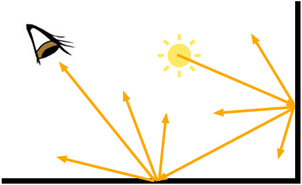
\includegraphics[width=0.45\textwidth]{images/path-tracing.png}
			\caption{
				\href{https://www.scratchapixel.com/lessons/3d-basic-rendering/global-illumination-path-tracing/introduction-global-illumination-path-tracing.html}{Схема траекторий движений лучей в методе трассировки путей}
			}
		\end{figure}

		\note{
			\footnotesize

			% \vspace{0.15cm}

			Шаги процесса

			1. Генерация первичных лучей. 
			
			2. Определение точек пересечения.
			
			3. Генерация дополнительных лучей.

			При этом используется случайное сэмплирование (Monte Carlo) для определения пути лучей, что позволяет учесть как прямое, так и косвенное освещение.

			% , при этом, если материал поверхности имеет ненулевую:
			% зеркальную составляющую, то генерируются отражённые лучи
			% прозрачную составляющую --- преломлённые лучи;
			% диффузную составляющую, то --- рассеянные лучи

			% 3. Определение вклада каждого источника света и многократных отражений на основе уравнения рендеринга за счет генерации дополнительных лучей

			т.о. цвет пикселя вычисляется на основе модели освещения, параметров источников света и свойств материала поверхности.
			
			

			4. Сборка итогового изображения

			Шаги с 1 по 3 повторяются, а результаты расчётов цветовых вкладов всех лучей усредняются по каждому пикселю.

			Чем больше лучей отправлено через пиксель, тем точнее и чище становится изображение (меньше шума).

		}


	\end{frame}

	\begin{frame}{Трассировка пути (Path Tracing)}

		\footnotesize

		\begin{itemize}

			\item 
			Метод Монте-Карло (Monte Carlo, 1949~г., Н. Метрополис и С. Улам)\\
			Семейство методов случайных выборок, разработанных для решения задач интеграции многомерных функций. Подходит для моделирования освещения в сложных сценах.\\
			{Источник:} \href{https://web.williams.edu/Mathematics/sjmiller/public_html/105Sp10/handouts/MetropolisUlam_TheMonteCarloMethod.pdf}{The Monte Carlo method, N. Metropolis и S. Ulam, 1949~г.}
			
			\item 
			Трассировка путей (Path Tracing, 1986~г., Джеймс Кадзия)\\
			Расширение трассировки лучей для симуляции глобального освещения. Впервые описано в статье «The Rendering Equation».\\
			{Источник:} «The Rendering Equation», J. Kajiya, 1986~г.
						
			\item 
			Реалистичные изображения в кинематографе (Path Tracing, 2000-е годы)\\
			Path Tracing активно использовался в анимационных фильмах, таких как «Скуби-Ду» и «В поисках Немо». Компания Pixar внесла значительный вклад в популяризацию технологии.\\
			{Источник:} Использование Path Tracing в индустрии анимации, 2000-е годы.
			
			\item 
			Path Tracing в реальном времени (Real-Time Path Tracing, 2020-е годы)\\
			Современные достижения позволили внедрить Path Tracing в игры. Реализация: Quake II RTX (2019), Portal RTX (2022), Cyberpunk 2077: Ray Tracing Overdrive (2023), Alan Wake 2 (2023) с DLSS 3.5 и другие проекты.\\
			{Источник:} NVIDIA RTX, разработчики игр и технологий, 2020-е годы.

		\end{itemize}

		\note{
			\footnotesize

		Главным недостатком является его	вычислительная стоимость, поскольку необходимости трассировать множество путей для каждого пикселя, особенно в сложных сценах, 
		и поэтому также применяются оптимизации:
			\begin{itemize}
				\item 
				Снижение шума (Denoising).\\
				Шум возникает при малом числе лучей. 
				Алгоритмы denoising (снижения шума) используют машинное обучение или другие статистические методы для удаления шума из промежуточных изображений.
				\item 
				Использование ускоряющих структур (Acceleration Structures).\\
				BVH (Bounding Volume Hierarchy) и KD-деревья — это методы для ускорения поиска пересечений лучей с объектами в сцене, за счет уменьшения проверок пересечений.
				\item 
				Выборка по значимости (Importance Sampling).\\
				Метод, при котором пути лучей выбираются с учетом их вероятности столкновения со значимыми источниками света.
				\item 
				Адаптивное сэмплирование (Adaptive Sampling).\\
				Метод, при котором количество сэмплов изменяется в зависимости от сложности сцены. 
			\end{itemize}


			

		}

	\end{frame}


	\if 0

	\begin{frame}{DLSS (Deep Learning Super Sampling) и FidelityFX Super Resolution (FSR) }

		% https://the-decoder.com/nvidias-dlss-3-5-brings-ai-rendered-ray-tracing-to-games-like-cyperpunk-2077/


		DLSS (Deep Learning Super Sampling, 2018 г.) --- технология от NVIDIA, использующая AI для повышения производительности и улучшения качества изображения в играх.

		\begin{itemize}
			\item[DLSS 1.0 (2018)] Основана на предварительно обученных нейронных сетях. Она увеличивала разрешение, но страдала от артефактов и размытых деталей, что вызвало критику.
			\item[DLSS 2.0 (2020)] Значительно улучшены качество изображения и универсальность. Технология стала более гибкой, поддерживая игры без необходимости специфической настройки. Она также снизила артефакты и обеспечила четкость изображения при высоких FPS.
			\item[DLSS 3.0 (2022)] Введены новые возможности, такие как создание кадров с использованием AI и улучшение производительности в реальном времени.
			\item[DLSS 3.5 (2022)] Дополнительные улучшения в качестве изображений и производительности, включая улучшение технологий рендеринга и повышение четкости изображения.
	\end{itemize}

		\note{
			https://dzen.ru/a/ZhPs-Fqf6GG8VQBC

			AMD предложила свою технологию повышения качества изображения под названием FidelityFX Super Resolution (FSR)

			FSR 1.0 (Июнь 2021)

    Простая технология пространственного апскейлинга.

		FSR 2.0 (Май 2022):

    Использует временной апскейлинг. Снижает шумы и сохраняет больше деталей.

		FSR 3.0 (Анонс 2023):
			
			Преимущества FSR перед DLSS:

			Совместимость. Работает не только на видеокартах AMD, но и на NVIDIA (включая GTX), а также на Intel GPU.
			
			Открытая платформа. AMD сделала FSR открытым стандартом, что облегчает внедрение в игры.
		
			Отсутствие зависимости от AI-ускорителей. FSR не требует специализированных тензорных ядер, как DLSS.

		}
		
	\end{frame}

	\begin{frame}{Физические модели}
		\begin{itemize}
			\item 
			Радиозити (Radiosity, 1950-е, Горацио Слоатер)\\
			Рассчитывает диффузное взаимное отражение между поверхностями.\\
			[Источник: Основы заложены в 1950-х, компьютерное применение — 1984]
			http://ray-tracing.ru/articles219.html

			\item 
			Фотонная карта (Photon Mapping, 1995 г., Хенрик Ванке)\\
			Двухпроходный алгоритм: накопление фотонов и рендеринг.\\
			[Источник: «Global Illumination Using Photon Maps», Henrik Wann Jensen, 1995]
		
			% \item 
		\end{itemize}
		
		\note{
			SSGI (Screen Space Global Illumination, 2010-е)\\
			Освещение на основе данных с экрана.\\
			[Источник: Используется в игровых движках, авторство технологии варьируется.]
			

			Радиозити (Radiosity, 1950-е)

			Диффузное взаимное освещение, основанное на принципах теплопередачи.
			Используется для статических сцен.
			Параллельное развитие:
			→ Фотонная карта (Photon Mapping, 1995):
			Двухэтапный алгоритм для более сложного освещения (например, каустики).

		}
	\end{frame}

	\begin{frame}{Метод фотонных карт}

		Метод фотонных карт --- метод глобального освещения, решающий задачу вычисления интеграла освещенности в самом общем случае. 
		
		\note{
			Алгоритм
	
			1. Фаза трассировки фотонов (Photon Tracing)
	
			Трассировка фотонов от источников света (физические лучи света).
			Каждый фотон рассекается или отражается от объектов в сцене, и его параметры (позиция, направление, цвет и интенсивность) записываются в структуру данных (photon map).
	
			2. Построение фотонной карты (Rendering Photon Mapping)
	
			Для каждого пикселя сцены трассируются лучи, и вычисляется освещённость, используя данные из photon map.
			Алгоритм использует данные из карты фотонов для аппроксимации взаимодействий света с поверхностями, что позволяет учитывать глобальное освещение (отражения, рассеяния, преломления и т.д.).
	
			3. Сбор освещенности
	
			Для каждого луча, который попадает в сцену, находится несколько ближайших фотонов в photon map, что позволяет оценить освещённость в данной точке.
			Используются различные методы поиска, такие как дерево k-Nearest Neighbors (k-NN), для ускорения процесса.

		}

	\end{frame}
		\fi
		
	
\end{document}